
\documentclass{beamer}
\usetheme{PaloAlto} %was Warsaw, Singapore, PaloAlto, Ilmenau, Boadilla
% see http://www.pletscher.org/writings/latex/beamerthemes.php
\usepackage{verbatim} %for comments
\usepackage[english]{babel}
\usepackage[latin1]{inputenc}
\usepackage{amsmath}
\usepackage{mathrsfs}
\usepackage{epsfig}
\usepackage{epic}
\usepackage{amsmath}
\usepackage{amsfonts}
\usepackage{amssymb}
\usepackage{latexsym}
\usepackage{multirow}
%\usepackage{algorithm}


\AtBeginSection[]
{
  \begin{frame}<beamer>
    \frametitle{Volume and Integration}
    \tableofcontents[currentsection,currentsubsection]
  \end{frame}
}


\begin{document}

\title{Latte Valuations: Volume and Integration}
\author{}
\date{\today}

\frame{\titlepage}

\section{Volume}




\frame{
\frametitle{Two Flavors}
Latte can compute normalized volumes of polytopes using two different methods:
\begin{enumerate}
\pause
\item The Triangulation Method: Triangulate the polytope into simplices, then use the determinant to find the volume of each simplex.
\pause
\item The Lawrence Method: Triangulate every vertex tangent-cone into simplicial cones and then use a volume formula by Jim Lawrence.
\end{enumerate}
}%frame

\subsection{Triangulation Algorithm}

\frame{
\frametitle{Volume of a square}
\begin{center}
\resizebox{1.5in}{!}{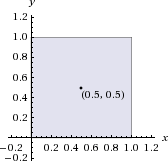
\includegraphics[]{img/unitSquare.png}}
\end{center}
Take the unit square centred at $(1/2, 1/2)$ above; after triangulation, we have two triangles: $\left\lbrace   (0, 0), (1, 0), (1, 1)\right\rbrace$ and $\left\lbrace  (0, 0), (0, 1), (1, 1)\right\rbrace$. Summing the determinant of tiangles' rays and dividing by two give the volume as 1.
}%frame


\frame{
\frametitle{Volume of a square}
\begin{center}
\resizebox{1.5in}{!}{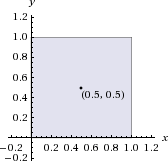
\includegraphics[]{img/unitSquare.png}}
\end{center}
In general, if $\left\lbrace (v_{0i}, v_{1i}, \ldots, v_{di})\right\rbrace  = T_i$ forms a d-simplex such that
the family $\left\lbrace T_1, \ldots, T_k \right\rbrace = \mathcal{T}$ is a triangulation of a d-Polytope, then the volume is given by:

$$
\sum_{T_i \in \mathcal{T}} |\det ( v_{1i} - v_{0i}, \ldots, v_{di} - v_{0i})| / d!
$$
}%frame

\subsection{Triangulation Example}
\frame{
\frametitle{Volume of a square}
For the first step in latte, we need create a file containing he hyperplanes that define the polytope. If $P = \left\lbrace x : Ax < b \right\rbrace$ for some $m \times n$ matrix $A$, then the input file will have the form:

$$
\begin{array}{l l}
 m & n + 1 \\
 \multicolumn{2}{l}{0 \leq b_{i} - a_{i}} \\

\end{array}
$$

where $b_{i}$ is the $i^{th}$ entry of b and $a_i$ is the $i^{th}$ row of $A$.
}%frame


\frame{
\frametitle{Volume of a square}
For our square, its defining hyperplanes are 
$$0 \leq x \leq 1, 0 \leq y \leq 1$$
and so we create a file that contains

\begin{block}<+->{square.latte}
	\begin{tabular}{rrr}
	4 &3 & \\
	0 &1 &0 \\
	1 &-1 &0 \\
	0 &0 &1 \\
	1 &0 &-1 \\
	\end{tabular}
\end{block}

}%frame



\frame{
\frametitle{Volume of a square}
Finally, the command we need is 

\begin{block}<+->{Command:}
./ValuationComputation  --valuation=volume --triangulate square.latte
\end{block}

\begin{block}<+->{Output:}
Volume (using the triangulation-determinant method) \\*
Answer: 1 (as a fraction) \\*
Decimal: 1 \\*
Time: 0.00 sec
\end{block}

}%frame

\subsection{Lawrence Algorithm}


\frame{
\frametitle{Volume of a Square}

Take the same unit square the Lawrence formula gives the volume in terms of the vertices and rays of every tangent cone. If the tangent cones are not simplicial, they must be first triangulated. For our square, the simplicial tangent cones are:

\begin{center}
\begin{tabular}{|c|c|}
	\hline
	Vertex & Rays \\
	\hline
	(0, 0) & (1, 0), (0, 1) \\
	(1, 0) & (-1, 0), (1, 0) \\
	(0, 1) & (0, -1), (-1, 0) \\
	(1, 1) & (-1, 0), (0, -1) \\
	\hline
\end{tabular}
\end{center}
}%frame


\frame{
\frametitle{Lawrence}
Let $v$ be a vertex of a d-polytope's vertex set $V$, and $\mathcal{T}_v = \left\lbrace T_{v_1}, \ldots, T_{v_i} \right\rbrace $ be a triangulation of the tangent cone at $v$. That is, each $T_{v_i} = \left\lbrace r_{1,v_i}, \ldots, r_{d,v_i} \right\rbrace $ is a set of d rays oriented from vertex $v$ to its adjacient vertices. Then the volume is given by 

$$
\sum_{v \in V} \sum_{T_{v_i} \in \mathcal{T}_v } \dfrac{\left\langle v, c\right\rangle ^d |\det{(r_{1, v_i}, \ldots, r_{d, v_i})|}} {\prod_{k = 1}^{k = d} \left\langle -r_{k, v_i}, c \right\rangle  }
$$

where $c$ is any random vector such that you do not divide by zero!
}%frame

\frame{
\frametitle{Volume of a square}
To use the Lawrence method on the square example:

\begin{block}<+->{Command:}
./ValuationComputation  --valuation=volume --lawrence square.latte
\end{block}

\begin{block}<+->{Output:}
Volume (using the Lawrence method) \\*
Answer: 1 (as a fraction) \\*
Decimal: 1 \\*
Time: 0.00 sec
\end{block}
}%frame



\frame{
\frametitle{Data Structures}

}%frame

\section{Integration}

\frame{
\frametitle{Algorithm}
\begin{itemize}
\item
\item
\end{itemize}
}%frame	

\frame{
\frametitle{Examples}
}%frame


\end{document}
